\chapter{Introduction}

Optimization problems can be described as trying to find the optimal solution while being under a set of constraints. Many problems that exist in the field of engineering and natural science can be categorized as optimization problems. A simple example might be mapping applications, which use an algorithm to find the shortest path between two points --- minimizing or optimizing the distance traveled --- while under constraints such as traffic laws or avoiding road work.

Gradient-based iterative algorithms are a tool to optimize large optimization problems. Their ability to efficiently optimize functions makes them extensively used in fields such as machine learning and data science \cite{Wright_Recht_2022}. There exist many different types of problems and many more methods that can be used to optimize them. Consequently, the ability to measure and compare the performance of algorithms can be helpful. It allows us to find the best-performing algorithm for any given problem category, improving efficiency and saving computation resources. As a result, substantial research has been conducted to quantify the performance of algorithms either through empirical evidence or mathematical proof.

Algorithm analysis is a field that seeks to prove a performance guarantee of an algorithm for solving a set of optimization problems. There are two approaches in the field, both of which arrive at the goal by solving an optimization problem and proving a performance rate mathematically. As a result, applying one of the methods in algorithm analysis often requires extensive knowledge of the field.

The main work of this thesis is the development of \texttt{AlgorithmAnalysis.jl}, a computer program written in the Julia programming language that applies the Lyapunov function-based approach to analyzing gradient-based algorithms. The package can automatically find the worst-case performance guarantee of an algorithm for a specified set of problems, making the analysis of iterative gradient-based methods accessible to a broad user base. After the program is given a class of functions and the algorithm to be analyzed, it returns a guaranteed rate at which the algorithm can optimize any function in the set.

%%%%%%%%%%%%%%%%%%%%%%%%%%%%%%%%%%%%%%%%%%%%%%%%%%%%%%%%%%%%%%%%%%%%%%%%%%%%%%%%
\section{Optimization problems and algorithms} \label{OpPro}

In this thesis, the optimization problem considered is in the form of finding the minimum point of a differentiable function:
\begin{subequations}\label{opt prob}
  \begin{align*}
    \textrm{minimize} &\quad f(x) \\
    \textrm{subject to} &\quad x \in X
  \end{align*}
\end{subequations}
where \(f(x)\) is the optimization function and \(X\) is a constraint set. Here, \(x\) is the input or decision/optimization variable, and \(f(x)\) is a measure of the cost or loss associated with each candidate solution $x$. Well-known examples of this problem are present in the training of large language models (LLMs) such as ChatGPT or the machine learning models that enable self-driving features in automobiles. An integral part of the training process of these models, through which they are created and continuously improved, is the minimizing of loss functions. In this process, a function is used to quantify the dissimilarity between a model's output and the desired values, and the model's parameters are modified iteratively using an algorithm in order to minimize the function and improve the model's performance.

While traversing any function can give its minimum, for large-scale and complex problems, it is more efficient to optimize functions numerically using iterative gradient-based algorithms. These algorithms minimize a function by starting at an initial point \(x_{0}\) and iteratively updating an estimate \(x_k\) (\(k\) representing the current iteration number), using the gradient of the function at each iteration $\nabla f(x_k)$ until it reaches a local minimum \(x_s\). For example, the gradient descent (GD) algorithm updates \(x_k\) following this formula:

\begin{equation}\label{eqn:GD}
  x_{k+1}=x_{k}-\alpha \nabla f(x_k)
\end{equation}

where $\alpha$ is the step size, an adjustable algorithm parameter. The stepsize $\alpha$ can affect the speed at which the algorithm converges, or whether it converges at all. Following this update formula, in each iteration, \(x\) moves toward the goal \(x_s\) where the gradient is zero $\nabla f(x_s) = 0$ and stays there afterward. Two areas where an algorithm like gradient descent can be improved are the number of iterations until the goal is reached, or the problem of overshooting, where the goal is not reached within an acceptable margin due to a step size too large. Accelerated algorithms exist that seek to overcome these problems, such as Polyak’s Heavy Ball (HB) method which introduces a momentum that incorporates previous iterations of \(x\) \cite{HB}:

\begin{equation}\label{eqn:HB}
  x_{k+1}=x_k-\alpha \nabla f(x_k)+ \beta (x_k-x_{k-1})
\end{equation}
where $\beta$ is another stepsize parameter, while Nesterov’s Fast Gradient (FG) method evaluates the gradient at an interpolated point \cite{FG}:
\begin{subequations} \label{eqn:FG}
  \begin{align}
    x_{k+1}     &=x_k-\alpha \nabla f(y_k), \label{eq_state}       \\
    y_{k+1} &=x_{k+1}+\beta (x_{k+1}-x_k) \label{eq_interpolated point}
  \end{align}
  \end{subequations}
In the rest of this thesis, we will use these three examples of iterative gradient-based algorithms to introduce the concept of algorithm analysis, the Lyapunov-based method, and how it is implemented.
%%%%%%%%%%%%%%%%%%%%%%%%%%%%%%%%%%%%%%%%%%%%%%%%%%%%%%%%%%%%%%%%%%%%%%%%%%%%%%%%
\section{Algorithm analysis}
Let us consider the problem of minimizing a simple quadratic function with no constraint:
\begin{equation} \label{eqn:quadratic}
    f(x) = x^2/2 - 3x + 4
\end{equation}
Using the (GD) equation \eqref{eqn:GD}, substituting step size $\alpha$ with values 0.2, 0.5, and 2, and picking a starting point of $x_0 = 0$, we will try to find the minimizer of this quadratic function. By counting the number of iterations each variation runs for before reaching 0.001 of the true minimum, we can measure the iteration complexity in \cref{fig:test}.

\begin{figure}[h!]
  \centering
  \begin{subfigure}{.5\textwidth}
    \centering
    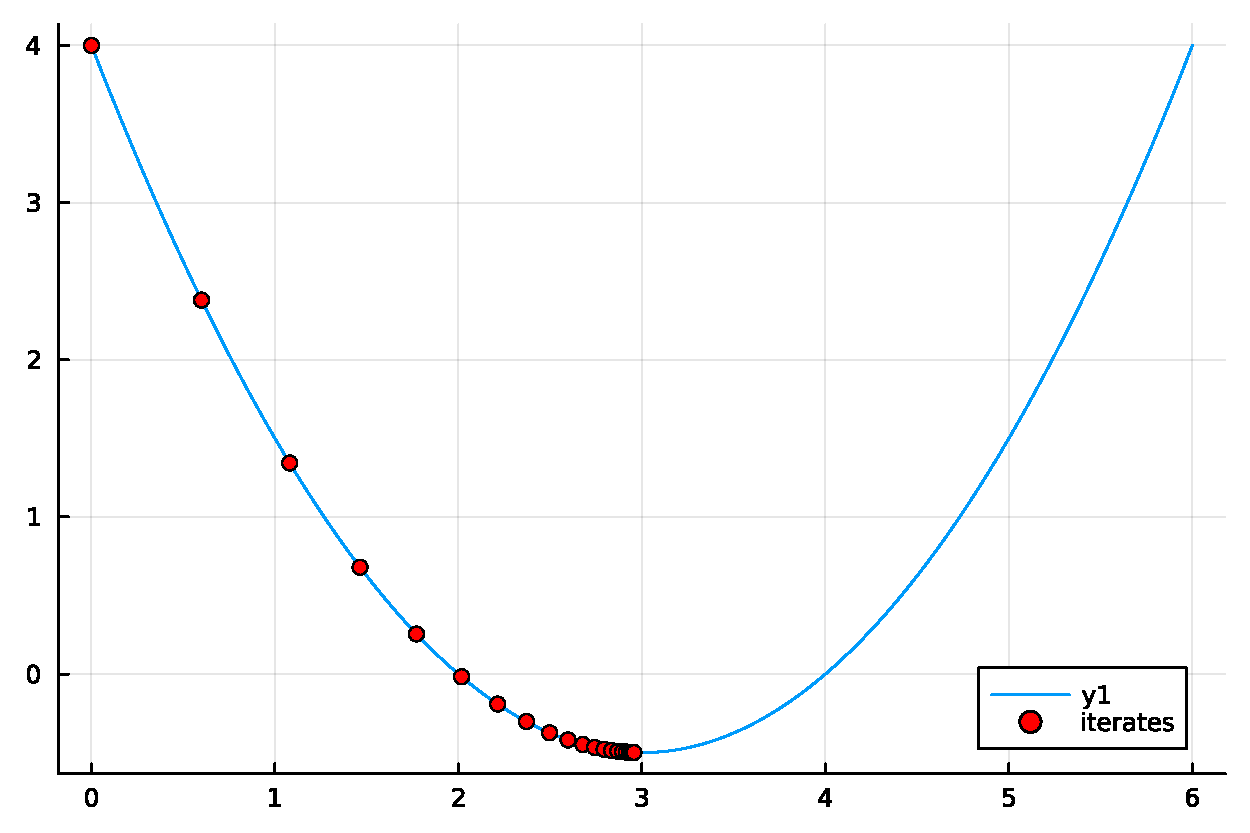
\includegraphics[width=.85 \linewidth]{crude1}
    \caption{$\alpha = 0.2$, iteration complexity = 20}
    \label{fig:crude1}
  \end{subfigure}%
  \begin{subfigure}{.5\textwidth}
    \centering
    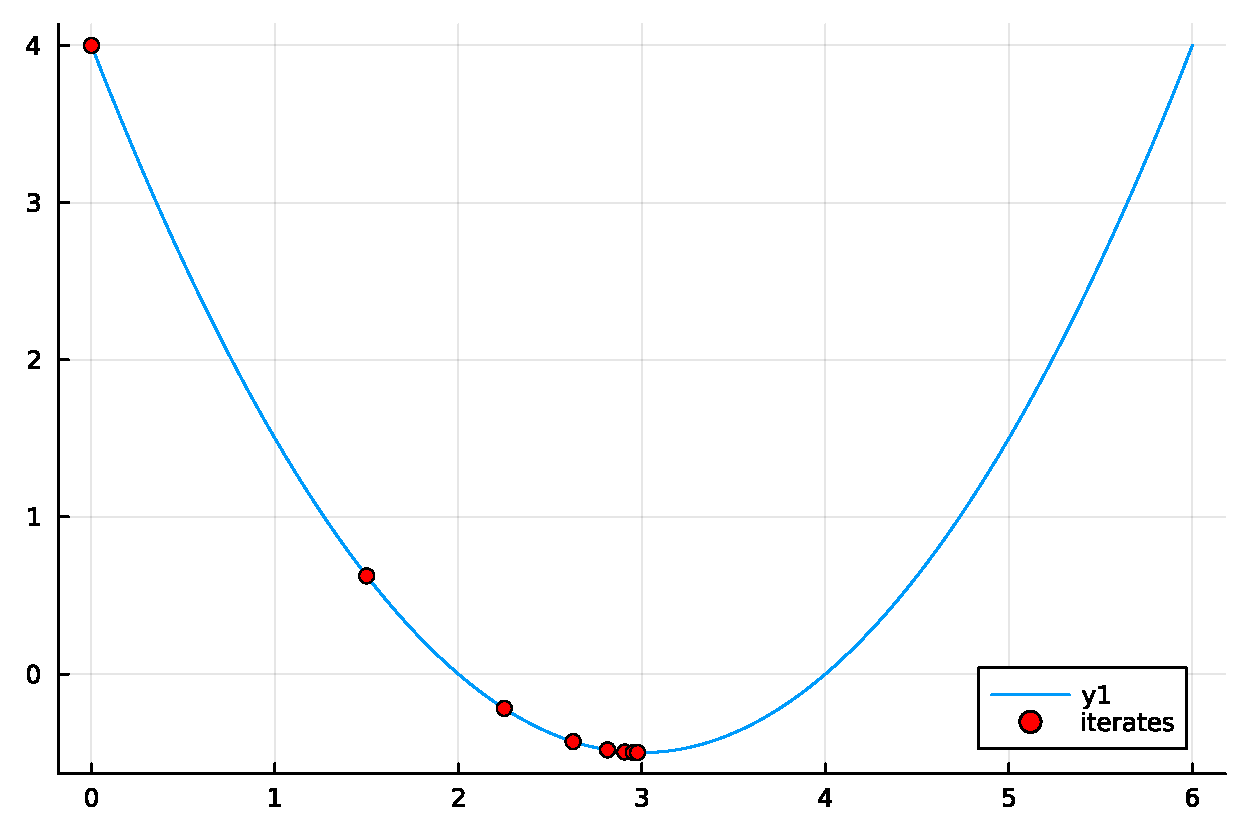
\includegraphics[width=.85 \linewidth]{crude2 }
    \caption{$\alpha = 0.5$, iteration complexity = 7}
    \label{fig:crude2}
  \end{subfigure}
  \begin{subfigure}{.5\textwidth}
    \centering
    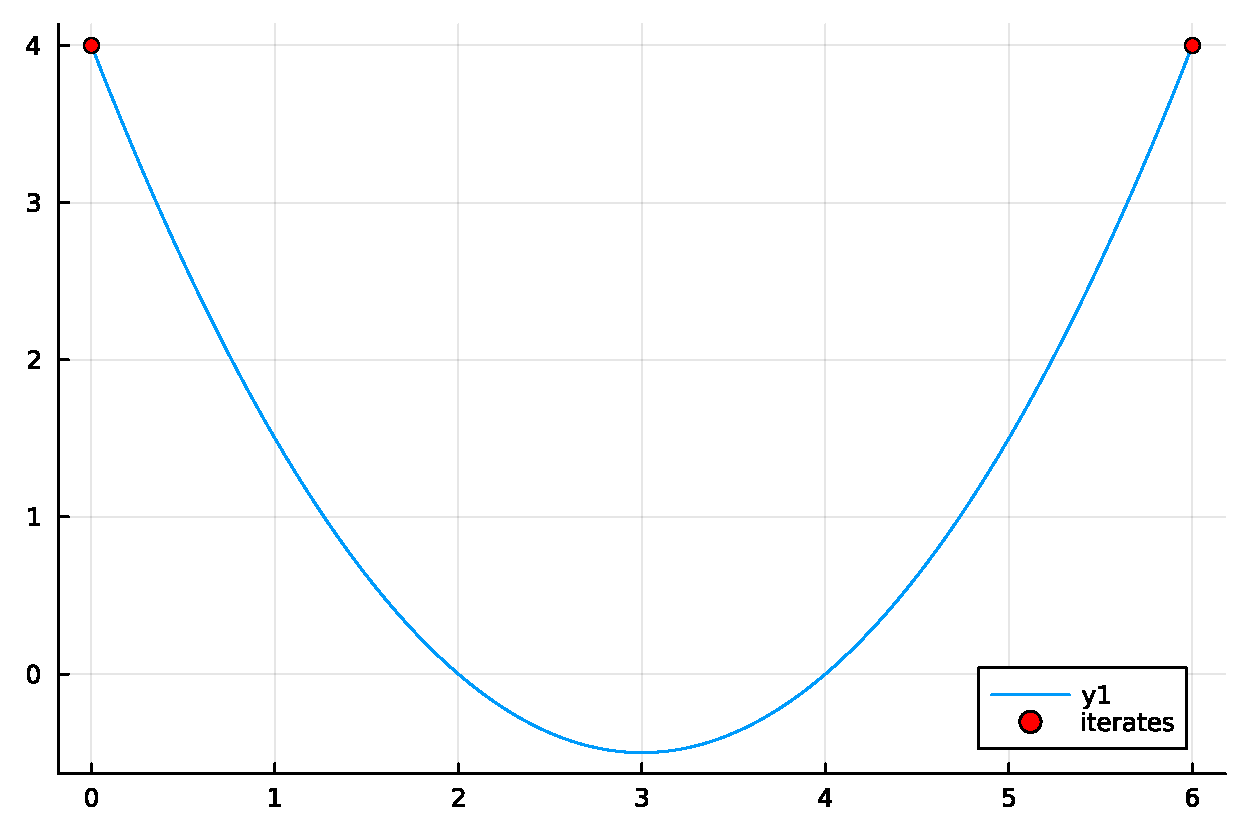
\includegraphics[width=.85 \linewidth]{crude3 }
    \caption{$\alpha = 2$, does not converge}
    \label{fig:crude3}
  \end{subfigure}
  \caption{Performance of 3 GD variants of different step sizes solving a quadratic function}
\label{fig:test}
\end{figure}

% \begin{figure}[htp]
%   \centering
%   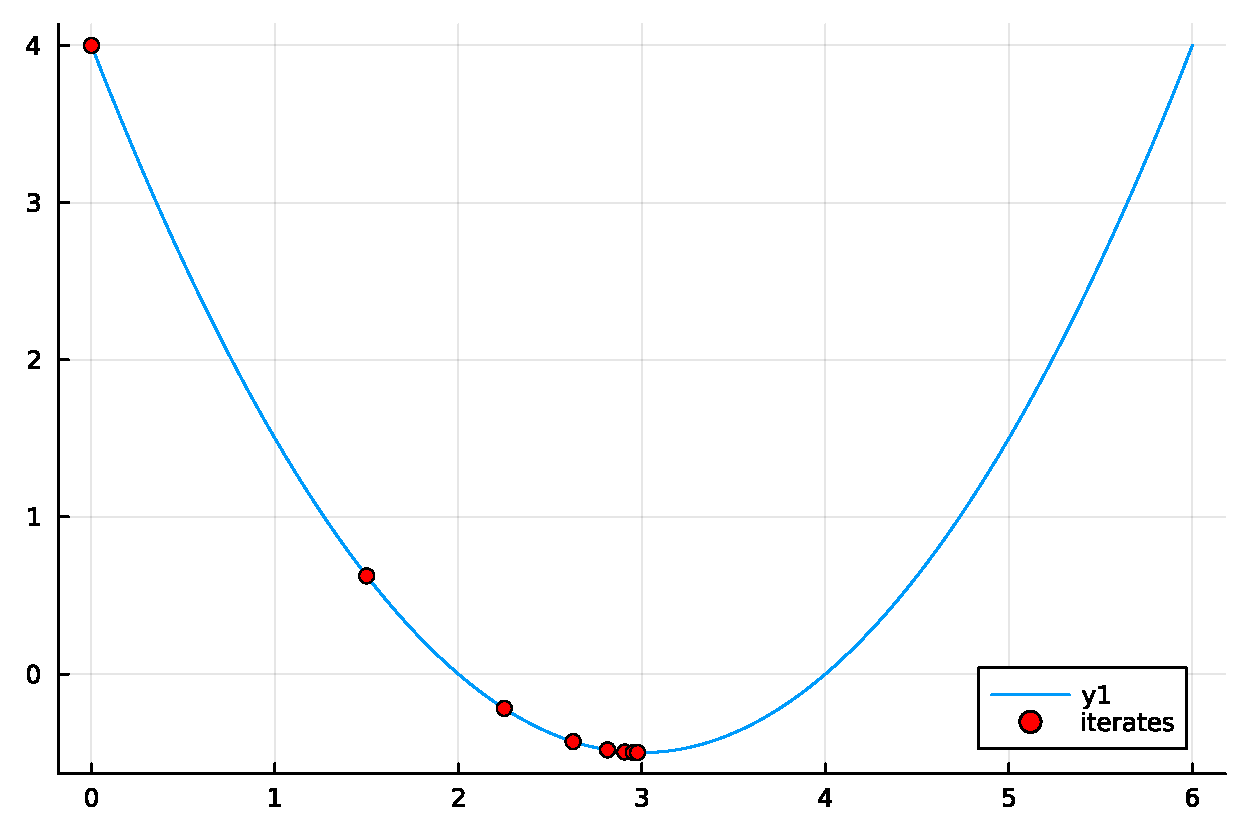
\includegraphics[width=.6\textwidth]{crude2}\hfill
%   \caption{$\alpha = 0.5$, iteration complexity = 21}
%   \label{fig:crude2}
% \end{figure}
% \begin{figure}[htp]
%   \centering
%   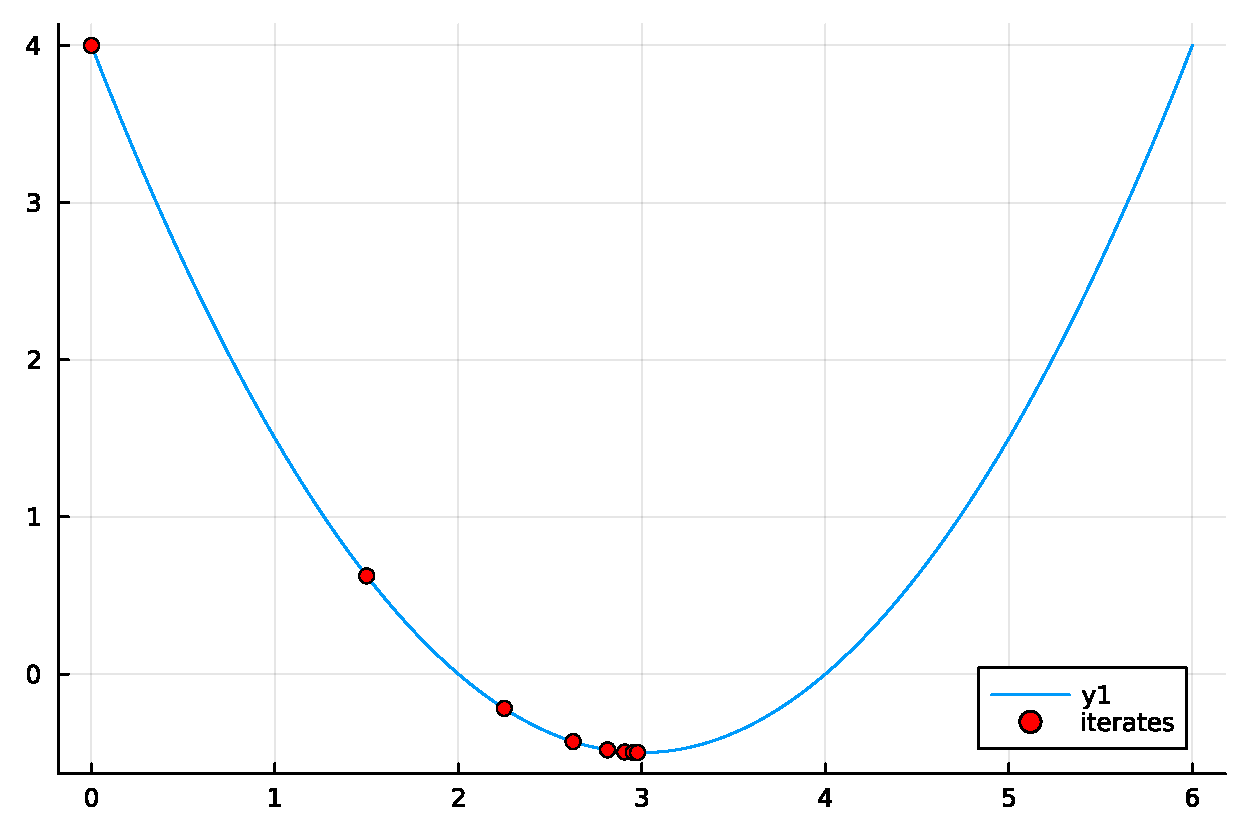
\includegraphics[width=.6\textwidth]{crude2}\hfill
%   \caption{$\alpha = 2$, does not converge}
%   \label{fig:crude3}
% \end{figure}

It can be seen how different tunings on the same algorithm can achieve drastically different speeds optimizing a function, or whether it can find the minimizer at all. Considering there exist many other first-order methods in addition to the three in \cref{OpPro}, each having infinitely adjustable parameters, finding the best algorithm for any problem set will mean it can optimized more quickly and more accurately.

While the analysis example in \cref{fig:test} yielded an analysis of the algorithms' performance, it required solving the optimization problem. Not only would solving any problem large enough to warrant being optimized numerically in the first place be computationally expensive, but any benefit of finding an algorithm superior at solving the problem is negated as it has already been solved. Additionally, any analysis result is applicable only to one function and cannot be reliably used to derive a first-order method's performance on any other problem.

In the application of training large language and self-driving models, the training process is continuous as more training data becomes available. This training uses vast amounts of time and computational power, and as a result, even a small improvement in the performance of the algorithm used can speed up the training process while reducing energy usage. However, as the problem becomes larger and more complex, so does the challenge of finding a better algorithm. It is more efficient therefore to analyze algorithms' performance at solving a broad set of problems.

As a result of their widespread application, popular iterative gradient-based algorithms have been extensively analyzed. A frequently cited attempt is the Adam algorithm \cite{adam}. Its author quantified and compared the performance of algorithms using experiments and empirical evidence. There exists a different approach, which measures the performance of an algorithm by mathematically proving a performance bound. This worst-case analysis is referred to as algorithm analysis: Given a characteristic that a set of functions might share (such as being convex or quadratic), it would return the worst-case performance measure that guarantees the algorithm analyzed would perform as well as or better at solving every function within said set.

\section{Julia programming language}

Our work uses the Julia programming language, a high-level programming language designed specifically for high-performance numerical computing. Julia's compiler performance has been benchmarked to be faster than many other languages used for numerical computing while being on par with C, a language often used for its high efficiency \cite{julia}. Julia accomplishes this while being a high-level language with simple syntax rules that resemble existing popular languages, making it easy to develop, use, and understand.

Julia is open-source and available for free on many popular platforms such as macOS, Windows, and Linux, making it a good choice for the \texttt{AlgorithmAnalysis.jl} package as it is designed with expert and novice users alike in mind.

Julia is also chosen as it is designed for numerical computing, supporting matrices as well as UTF-8 encoding, making it possible to use scientific notation: variables and functions as they exist in the code and as the user inputs them into the program can use math symbols or Greek letters. This makes Julia excel at communicating mathematical concepts, which simplifies both the process of coding the program and understanding its mathematical underpinnings. \cref{ex_analysis} shows sample code of how the package can be used, while \cref{chapter:code} explains our work's core code components.

\section{Analysis example}
To analyze the performance of an algorithm using the \texttt{AlgorithmAnalysis.jl} package, the user needs to follow the following 3 steps:
\begin{enumerate}
	\item Choose from a supported list the class of function to be optimized.
	\item Define an algorithm to be analyzed .
	\item Specify a performance measure.
\end{enumerate}
Our package defines a function class as every function that shares a trait. In example \cref{ex_analysis}, the class of function is $m$ smooth---$L$ strongly convex functions. Our work shares the notation and definition of smooth strongly convex functions with \cite{tutorial}, which uses the notation $F_{m,L}$ and defines the function class as any continuously differentiable functions that satisfy:
\begin{enumerate}
	\item $L$-Lipschitz gradients: $\|\nabla f(x) - \nabla f(x)\| \leq L\|x-y\|$ for all $x, y \in \mathbb{R}$.
	\item $m$-strong convexity: $f(x) - \frac{m}{2}\|x\|^2$ is convex.
\end{enumerate}
% \begin{equation}
%   (\nabla f(x) - m(x-x_*))^\tp (\nabla f(x) - L(x-x_*)) \leq 0
% \end{equation}
% where $x_*$ is the global minimum of the function $f$ for all x.

\begin{figure}[h!]
	\begin{lstlisting}[mathescape]
m,L = 1,10
$ \alpha $ = 2/(L+m)
@algorithm begin

	f = DifferentiableFunctional{R$ ^n $}() 
	xs = first_order_stationary_point(f)
	f $ \in $ SmoothStronglyConvex(m, L)

	x0 = R$ ^n $()
	x1 = x0 - $ \alpha $*f'(x0)

	x0 => x1

	performance = (x0-xs)^2
end

@show rate(performance)
\end{lstlisting}
\caption{Analysis example}
\label{ex_analysis}
\end{figure}

In the example code, the user:
\begin{itemize}
	\item Defines the class of function \texttt{f} and its gradient $\nabla f$, coded as \texttt(f') by calling the provided functions \texttt{DifferentiableFunctional} and \texttt{SmoothStronglyConvex}.
	\item Defines an initial state $ x_0 $ and how the algorithm creates the next state $ x_1$. In this example, the algorithm being analyzed is gradient descent with a step size $ \alpha = 2/11$.
	\item Sets the performance measure as the norm distance between the initial state and the goal $ (x_0 - x_s)^2 $. The returned convergence rate guarantee is the rate at which the performance measure decreases after each iteration of the algorithm.
	\item Call the rate function to start the analysis.
\end{itemize}

With the calling of the rate function, the program runs automatically to return a rate of 0.8176803588867188. This is the convergence rate guarantee $\rho$ such that, for some performance measure $c>0$, it is upper bounded by $c \rho^k$ at each iteration $k$, for the provided algorithm and every function in the class.

This guaranteed convergence rate using ``big O'' notation means that the performance measure converges with a minimum rate of $O(\rho^k)$. Throughout the process, the user never has to modify the package beyond providing its input or understand how the package \texttt{AlgorithmAnalysis.jl} operates.

\begin{figure}[hbtp]
  \begin{lstlisting}
  rate(performance) = 0.8176803588867188
  \end{lstlisting}
  \caption{Analysis result}
  \label{ex_result}
\end{figure}

\section{Overview} \label{sectionOverview}

% JuPE performs worst-case algorithm analysis when three main inputs are provided: the class of functions in question, the algorithm being analyzed, and a performance measure. The package then performs the algorithm analysis and returns the fastest guaranteed convergence rate.

% To use JuPE, an iterative first-order algorithm needs to be defined as an input to the program by specifying how it is updated. The class of function is provided by detailing the characteristic of the set, and a performance measure is defined. Throughout the process, the user never has to change the code of the package or understand how JuPE works, making it an easy to use black box tool.

%, such as 1 strong 10 smooth convex function, which can be how far the iterate \(x_k\) is from the goal \(x_*\) or any quadratic combinations of the iterates
After the introduction, in \Cref{chapter:literature}, the existing literature on analyzing algorithms is presented. \Cref{chapter:lyapunov} discusses the Lyapunov-based mathematical method that \texttt{Algorithm\allowbreak Analysis.jl} utilizes. \Cref{chapter:code} demonstrates the domain-specific language developed and how it supports the package's functionality. \Cref{chapter:process} details the analysis process. Analysis results produced by the package is presented in \cref{chapter:results}. Finally, discussion about the package and potential future work and our conclusion is presented in \cref{chapter:conclusion}.

% \comment{Reference the specific chapters, such as Chapter~\ref{chapter:literature} (see the reference label at the beginning of that chapter for how to make the rerence).}